\documentclass[a4paper,12pt,twoside]{article}
\usepackage{xcolor}
\definecolor{verde}{rgb}{0,0.5,0}
\definecolor{jpurple}{rgb}{0.5,0,0.35}
\usepackage[utf8]{inputenc}
\usepackage{graphicx}
\usepackage{float}
\usepackage[brazilian]{babel}
\usepackage{indentfirst}
\usepackage{steinmetz}
\usepackage{multicol}
\usepackage[left=2cm, right=2cm, top=2cm]{geometry}
\setlength\parindent{1cm}
\usepackage{mathrsfs, amsmath}
\usepackage{textcomp}
\usepackage{gensymb}
\usepackage{lipsum}
\usepackage{natbib}
\usepackage{listings}
\lstset{
  language=vhdl,
  basicstyle=\ttfamily\small, 
  keywordstyle=\color{blue}, 
  stringstyle=\color{verde}, 
  commentstyle=\color{red}, 
  extendedchars=true, 
  showspaces=false, 
  showstringspaces=false, 
  numbers=left,
  numberstyle=\tiny,
  breaklines=true, 
  backgroundcolor=\color{jpurple!10},
  breakautoindent=true, 
  captionpos=b,
  xleftmargin=0pt,
}

\headheight = 10pt

\setcounter{section}{-1}



\date{}

\begin{document}

\begin{titlepage}
\begin{center}
{\large Universidade Federal do Rio de Janeiro}\\[0.2cm]
{\large Engenharia Eletrônica e de Computação}\\[0.2cm]
{\large Trabalho de Sistemas Digitais}\\[5.1cm]
{\bf \huge ULA - Unidade Lógica Aritmética - 1° Trabalho}\\[5.1cm]
\end{center}
{\large Alunos(as): Gabriel de Lima Moura e Karen dos Anjos Arcoverde}\\[0.7cm]
{\large Professor: Luís Henrique Maciel Kosmalski Costa}\\[5.1cm]
\begin{center}
{\large Rio de Janeiro}\\[0.2cm]
{\large 2019.2}
\end{center}
\end{titlepage}

\renewcommand{\contentsname}{Sumário}

\tableofcontents
\clearpage


\section{Introdução}
Este trabalho tem como objetivo o desenvolvimento de uma Unidade Lógica e Aritmética (ULA) composta por 8 funções e com 2 entradas e 1 saída de 4 bits cada, além de 4 saídas para indicar flags (overflow, negativo, zero e carry out). 
A ULA foi feita em VHDL e implementada em uma placa FPGA e é composta pelas seguintes funções: \\ \\
 \begin{itemize}
   \item AND
   \item OR
   \item XOR
   \item NOT
   \item Somador de 4 bits
   \item Subtrator de 4 bits
   \item Coomplemento de 2
   \item Incremento
 \end{itemize}


\section{Funcionamento}
Para o projeto ser funcional na placa FPGA, alguns módulos especiais foram criados. \\ \\
As entradas da ULA são geradas por um módulo contador de 10 bits, que usa 8 bits para as 2 entradas e os 2 bits restantes para um vetor  usado para selecionar a saída que será mostrada nos leds da placa. 
\\ \\ Usaremos 6 leds na placa, 4 deles irão alternar(conforme a passagem de clock) entre as 2 entradas de 4 bits(para indicar quais entradas estã sendo utilizadas no momento), a saída(resultado) e as 4 flags compactadas em um vetor. Para a visualização das operações e os outros 2 irão indicar o que os 4 leds estão mostrando no momento, através dos 2 bits restantes do contador.  \\ \\
Os botões da placa são usados para fazer a seleção da operação a ser executada. A partir daí, os dados são passados para o módulo principal que analisa as entradas e executa as funções necessárias, além de mandar as saídas para os leds da placa.  \\ \\
    Na figura abaixo, esquematizamos como ocorre a relação entre as operações e os módulos.

\begin{figure}[H]
\centering
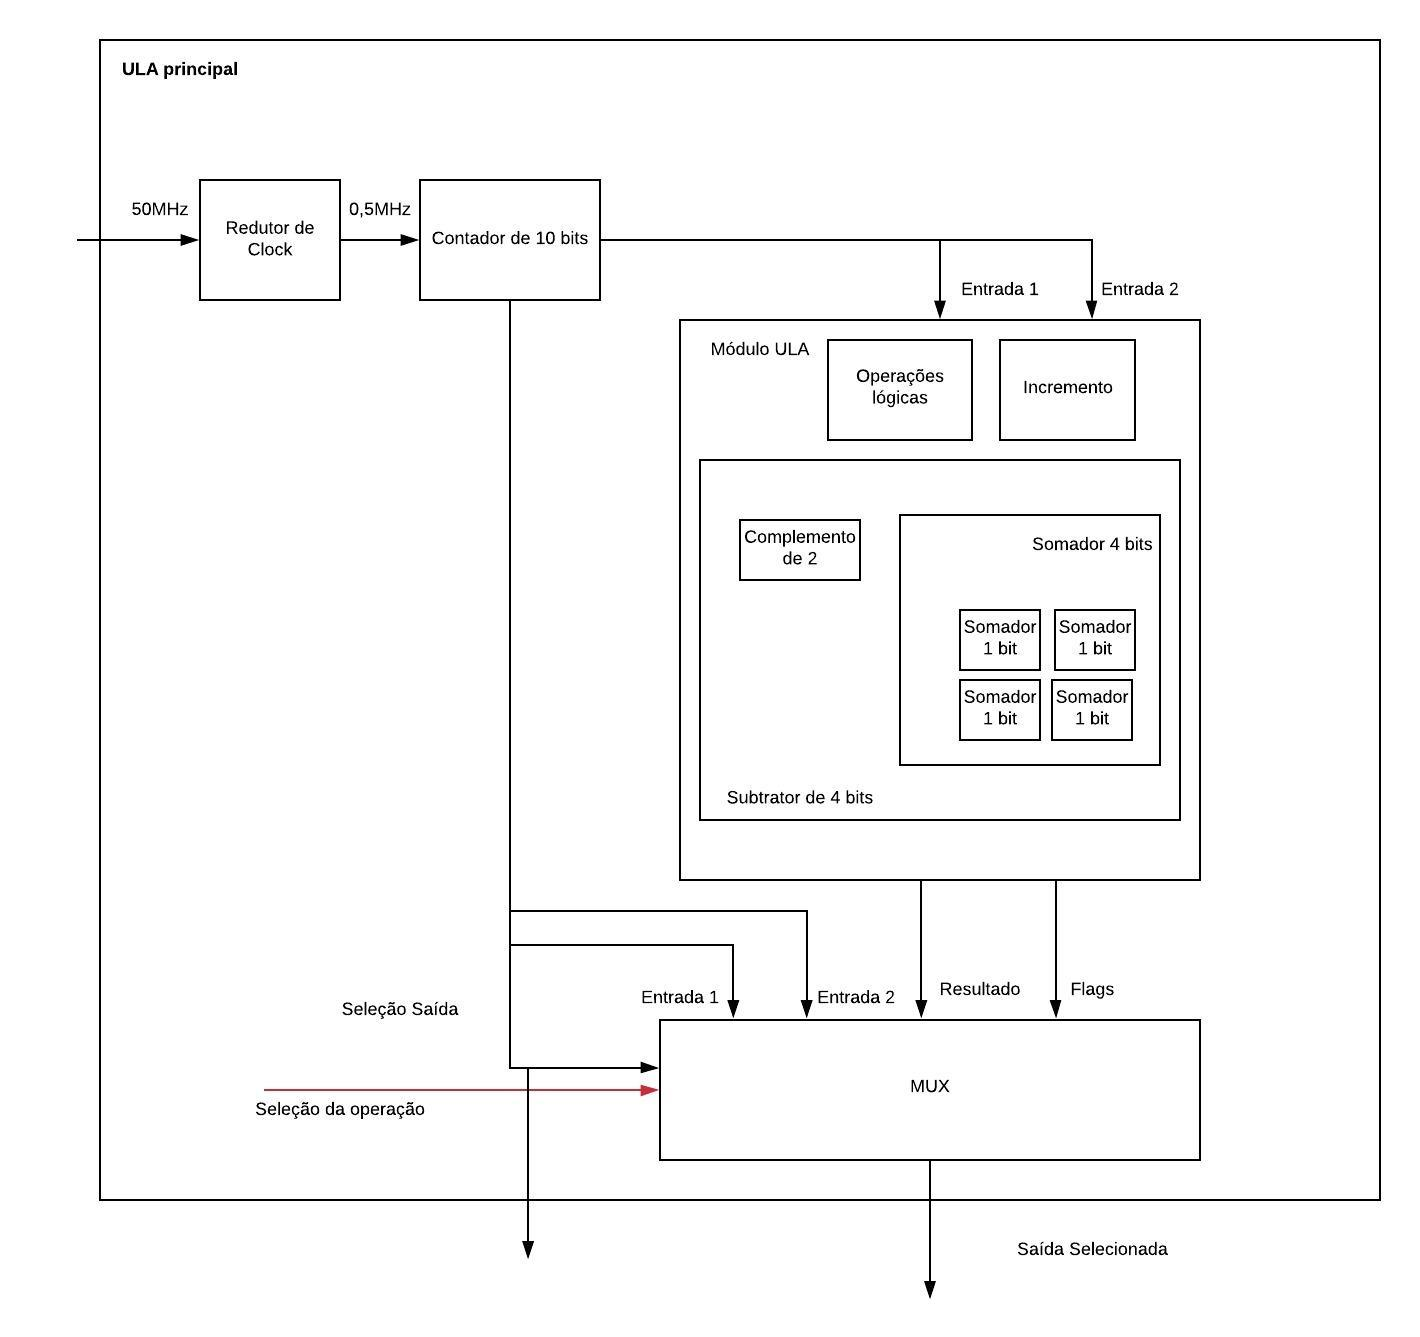
\includegraphics[scale=0.8]{diagrama.jpeg}
\caption{Diagrama de Blocos da ULA}
\label{fig:diagrama}
\end{figure}




%%%%%%%%%%%%%%%%%%%%%%%%%%%%%%%%%%%%%%%%%%%%%%%%%%%%%%%%%%%%%%%%%%%%%%%%%%%%%%%%%%%%%%%
\section{Funções}
%%% SOMADOR 1 BIT
\subsection{Somador de 1 bit}
    Este módulo recebe 2 entradas(A e B) de 1 bit e gera como saída o resultado da soma A + B.
    
\begin{lstlisting}
library IEEE;
use IEEE.STD_LOGIC_1164.ALL;

entity somador_1bit is
    Port ( entrada_1_s1bit : in  STD_LOGIC;
           entrada_2_s1bit : in  STD_LOGIC;
           cin_s1bit : in  STD_LOGIC;
           cout_s1bit : out  STD_LOGIC;
           soma_s1bit : out  STD_LOGIC);
end somador_1bit;

architecture Behavioral of somador_1bit is

begin

 cout_s1bit <= ((entrada_1_s1bit AND cin_s1bit) OR (entrada_2_s1bit AND cin_s1bit) OR (entrada_1_s1bit AND entrada_2_s1bit));
 soma_s1bit <= ((entrada_1_s1bit XOR entrada_2_s1bit) XOR cin_s1bit);

end Behavioral;
 } \end{lstlisting}
 
  \begin{figure}[H]
\centering
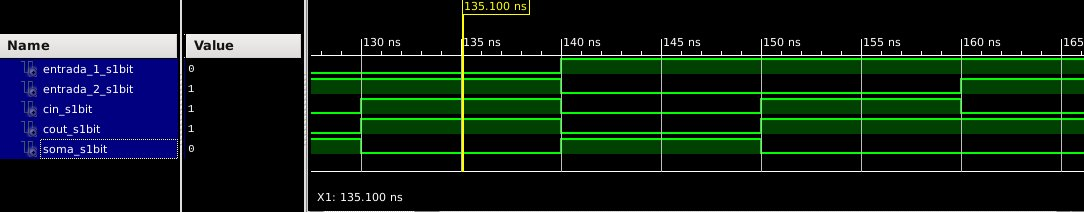
\includegraphics[scale=0.55]{testes/somador1bit.jpeg}
\caption{teste da função SOMADOR 1 BIT}
\label{fig:diagrama}
\end{figure}

 
%%% PORTA AND
\subsection{AND}
Recebe 2 entradas de 4 bits e gera o resultado da operação lógica (A)AND(B).

\begin{lstlisting}
library IEEE;
use IEEE.STD_LOGIC_1164.ALL;

entity porta_and is
    Port ( entrada_1_and : in  STD_LOGIC_VECTOR (3 downto 0);
           entrada_2_and : in  STD_LOGIC_VECTOR (3 downto 0);
           resultado_and : out  STD_LOGIC_VECTOR (3 downto 0));
end porta_and;

architecture Behavioral of porta_and is

begin

resultado_and <= ((entrada_1_and)AND(entrada_2_and));

end Behavioral;

 } \end{lstlisting}
 
 \begin{figure}[H]
\centering
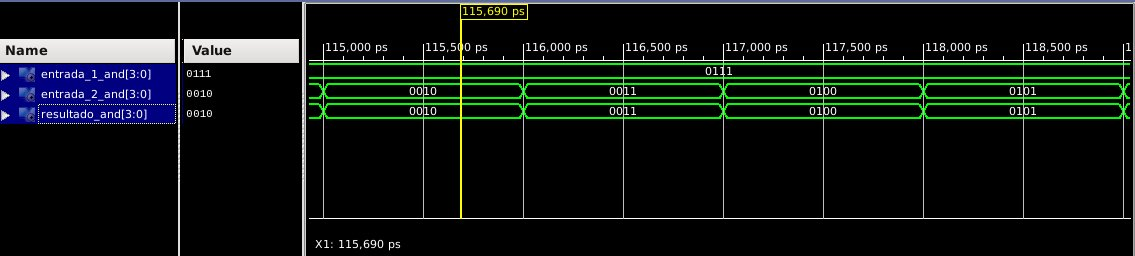
\includegraphics[scale=0.55]{testes/AND2.jpeg}
\caption{teste da função AND}
\label{fig:diagrama}
\end{figure}

 
 
%%% PORTA OR
\subsection{OR}
Recebe 2 entradas de 4 bits e gera o resultado da operação lógica (A)OR(B).

\begin{lstlisting}
library IEEE;
use IEEE.STD_LOGIC_1164.ALL;

entity porta_or is
    Port ( entrada_1_or : in  STD_LOGIC_VECTOR (3 downto 0);
           entrada_2_or : in  STD_LOGIC_VECTOR (3 downto 0);
           resultado_or : out  STD_LOGIC_VECTOR (3 downto 0));
end porta_or;

architecture Behavioral of porta_or is

begin

resultado_or <= ((entrada_1_or)OR(entrada_2_or));

end Behavioral;
 } \end{lstlisting}
 
  \begin{figure}[H]
\centering
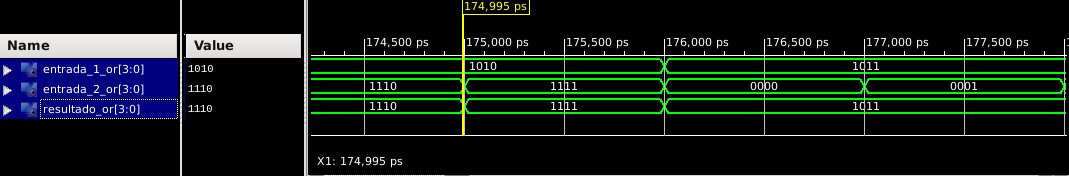
\includegraphics[scale=0.6]{testes/or2.jpeg}
\caption{teste da função OR}
\label{fig:diagrama}
\end{figure}
 
 
%%% PORTA XOR
\subsection{XOR}
Recebe 2 entradas de 4 bits e gera o resultado da operação lógica (A)XOR(B).

\begin{lstlisting}
library IEEE;
use IEEE.STD_LOGIC_1164.ALL;

entity porta_xor is
    Port ( entrada_1_xor : in  STD_LOGIC_VECTOR (3 downto 0);
           entrada_2_xor : in  STD_LOGIC_VECTOR (3 downto 0);
           saida_xor : out  STD_LOGIC_VECTOR (3 downto 0));
end porta_xor;

architecture Behavioral of porta_xor is

begin

saida_xor <= ((entrada_1_xor)XOR(entrada_2_xor));

end Behavioral;
 } \end{lstlisting}
 
   \begin{figure}[H]
\centering
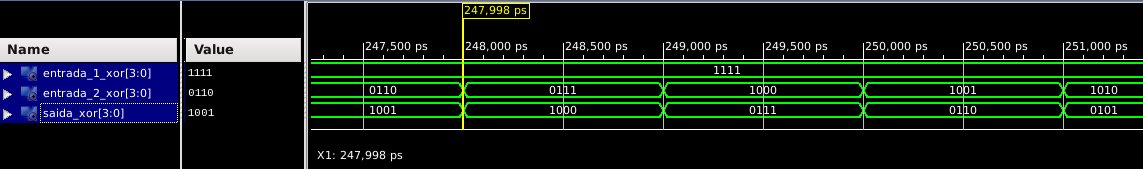
\includegraphics[scale=0.55]{testes/xor2.jpeg}
\caption{teste da função XOR}
\label{fig:diagrama}
\end{figure}

%%% PORTA NOT
\subsection{NOT}
Recebe 1 entrada de 4 bits e gera o resultado da operação lógica NOT(A).

\begin{lstlisting}
library IEEE;
use IEEE.STD_LOGIC_1164.ALL;

entity porta_not is
    Port ( entrada_not : in  STD_LOGIC_VECTOR (3 downto 0);
           saida_not : out  STD_LOGIC_VECTOR (3 downto 0));
end porta_not;

architecture Behavioral of porta_not is

begin

saida_not <= NOT(entrada_not);

end Behavioral;
 } \end{lstlisting}
   \begin{figure}[H]
\centering
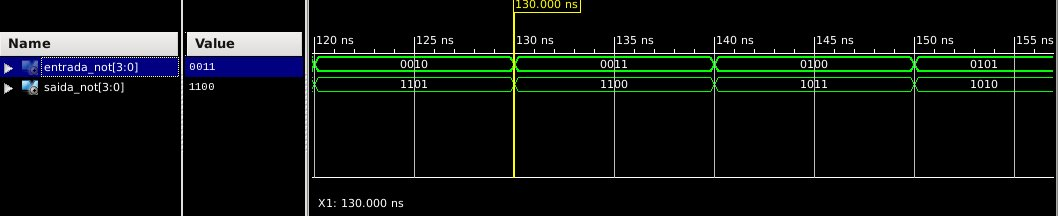
\includegraphics[scale=0.6]{testes/NOT2.jpeg}
\caption{teste da função NOT}
\label{fig:diagrama}
\end{figure}

%%% SOMADOR 4 BITS
\subsection{Somador de 4 bits}
Recebe 2 entradas de 4 bits e gera o resultado da operação  (A)+(B) além de 4 flags  correspondentes (OV , Neg, Cout, Zero).

\begin{lstlisting}
library IEEE;
use IEEE.STD_LOGIC_1164.ALL;

entity somador_4bits is
    Port ( entrada_1_s4bits : in  STD_LOGIC_VECTOR (3 downto 0);
           entrada_2_s4bits : in  STD_LOGIC_VECTOR (3 downto 0);
           cin_s4bits : in  STD_LOGIC;
           cout_s4bits : out  STD_LOGIC;
           soma_s4bits : out  STD_LOGIC_VECTOR (3 downto 0);
           overflow_s4bits : out  STD_LOGIC;
           negativo_s4bits : out  STD_LOGIC;
           zero_s4bits : out  STD_LOGIC);
end somador_4bits;

architecture Behavioral of somador_4bits is

component somador_1bit is
     Port ( entrada_1_s1bit : in  STD_LOGIC;
           entrada_2_s1bit : in  STD_LOGIC;
           cin_s1bit : in  STD_LOGIC;
           cout_s1bit : out  STD_LOGIC;
           soma_s1bit : out  STD_LOGIC);
end component somador_1bit;

signal conexao0 , conexao1 , conexao2 , cout_aux: STD_LOGIC;
signal soma_aux	:STD_LOGIC_VECTOR (3 downto 0);



begin
label0: somador_1bit port map(entrada_1_s4bits(0),entrada_2_s4bits(0),cin_s4bits,conexao0,soma_aux(0));
label1: somador_1bit port map(entrada_1_s4bits(1),entrada_2_s4bits(1),conexao0,conexao1,soma_aux(1));
label2: somador_1bit port map(entrada_1_s4bits(2),entrada_2_s4bits(2),conexao1,conexao2,soma_aux(2));
label3: somador_1bit port map(entrada_1_s4bits(3),entrada_2_s4bits(3),conexao2,cout_aux,soma_aux(3));


overflow_s4bits <= ((conexao2)XOR(cout_aux));
negativo_s4bits <= soma_aux(3);
zero_s4bits <= '1' WHEN (soma_aux = "0000")
		ELSE '0';
cout_s4bits <= cout_aux;
soma_s4bits <= soma_aux;

end Behavioral;
 } \end{lstlisting}
 
   \begin{figure}[H]
\centering
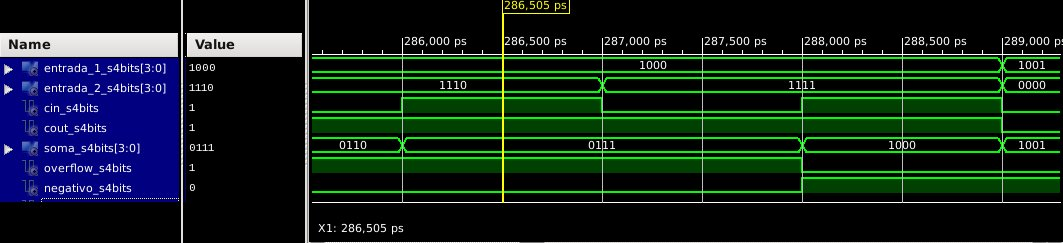
\includegraphics[scale=0.6]{testes/somador2.jpeg}
\caption{teste da função SOMADOR 4 BITS}
\label{fig:diagrama}
\end{figure}
 
 
%%% SUBTRATOR
\subsection{Subtrator de 4 bits}
Recebe 2 entradas de 4 bits e gera o resultado da operação  (A)-(B) além de 4 flags correspondentes (OV , Neg, Bout, Zero).

\begin{lstlisting}
library IEEE;
use IEEE.STD_LOGIC_1164.ALL;

entity subtrator_4bits is
    Port ( entrada_1_subt4bits : in  STD_LOGIC_VECTOR (3 downto 0);
           entrada_2_subt4bits : in  STD_LOGIC_VECTOR (3 downto 0);
           borrow_in_subt4bits : in  STD_LOGIC;
           borrow_out_subt4bits : out  STD_LOGIC;
           resultado_subt4bits : out  STD_LOGIC_VECTOR (3 downto 0);
           zero_subt4bits : out  STD_LOGIC;
           negativo_subt4bits : out  STD_LOGIC;
           overflow_subt4bits : out  STD_LOGIC);
end subtrator_4bits;

architecture Behavioral of subtrator_4bits is


component somador_4bits is
      Port ( entrada_1_s4bits : in  STD_LOGIC_VECTOR (3 downto 0);
           entrada_2_s4bits : in  STD_LOGIC_VECTOR (3 downto 0);
           cin_s4bits : in  STD_LOGIC;
           cout_s4bits : out  STD_LOGIC;
           soma_s4bits : out  STD_LOGIC_VECTOR (3 downto 0);
           overflow_s4bits : out  STD_LOGIC;
           negativo_s4bits : out  STD_LOGIC;
           zero_s4bits : out  STD_LOGIC);
end component somador_4bits;

signal cout_aux :STD_LOGIC;

begin
label0: somador_4bits port map(entrada_1_subt4bits , NOT(entrada_2_subt4bits) , '1' , cout_aux , resultado_subt4bits , overflow_subt4bits , negativo_subt4bits , zero_subt4bits);   
borrow_out_subt4bits <= NOT(cout_aux);

end Behavioral;
 } \end{lstlisting}
   \begin{figure}[H]
\centering
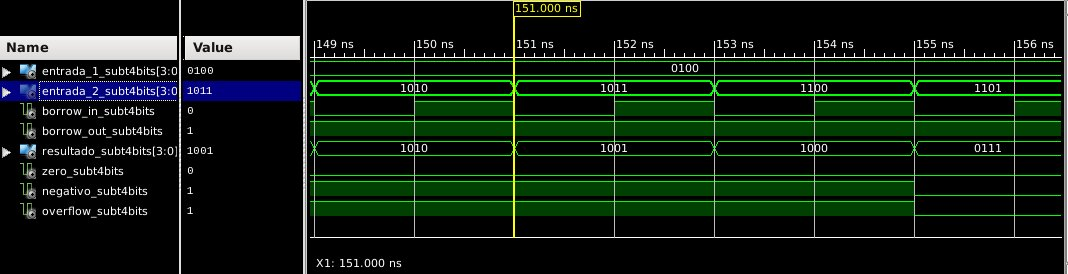
\includegraphics[scale=0.6]{testes/SUBTRATOR2.jpeg}
\caption{teste da função SUBTRATOR 4 BITS}
\label{fig:diagrama}
\end{figure}

%%% COMPLEMENTO DE 2
\subsection{Complemento de 2}
Recebe 1 entrada de 4 bits e gera o resultado da operação de complemento de 2 de A.

\begin{lstlisting}
library IEEE;
use IEEE.STD_LOGIC_1164.ALL;

entity complemento_2 is
    Port ( entrada_compl2 : in  STD_LOGIC_VECTOR (3 downto 0);
           saida_compl2 : out  STD_LOGIC_VECTOR (3 downto 0));
end complemento_2;

architecture Behavioral of complemento_2 is

component somador_4bits is
      Port ( entrada_1_s4bits : in  STD_LOGIC_VECTOR (3 downto 0);
           entrada_2_s4bits : in  STD_LOGIC_VECTOR (3 downto 0);
           cin_s4bits : in  STD_LOGIC;
           cout_s4bits : out  STD_LOGIC;
           soma_s4bits : out  STD_LOGIC_VECTOR (3 downto 0);
           overflow_s4bits : out  STD_LOGIC;
           negativo_s4bits : out  STD_LOGIC;
           zero_s4bits : out  STD_LOGIC);
end component somador_4bits;

signal cout_nao_usado , overflow_nao_usado , negativo_nao_usado , zero_nao_usado :STD_LOGIC ;

begin

label0: somador_4bits port map(NOT(entrada_compl2),"0001",'0',cout_nao_usado,saida_compl2,overflow_nao_usado,negativo_nao_usado,zero_nao_usado);

end Behavioral;
 } \end{lstlisting}
 
   \begin{figure}[H]
\centering
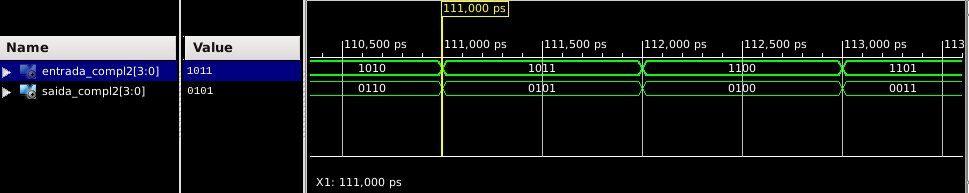
\includegraphics[scale=0.65]{testes/complemento_2_2.jpeg}
\caption{teste da função COMPLEMENTO DE 2}
\label{fig:diagrama}
\end{figure}

%%% INCREMENTO
\subsection{Incremento}
Recebe 1 entrada de 4 bits e gera o resultado da operação (A)+(0001) além das 4 flags correspondentes (OV , Neg, Cout, Zero).

\begin{lstlisting}
library IEEE;
use IEEE.STD_LOGIC_1164.ALL;

entity operacao_incremento is
    Port ( entrada_incremento : in  STD_LOGIC_VECTOR (3 downto 0);
           saida_incremento : out  STD_LOGIC_VECTOR (3 downto 0);
           negativo_incremento : out  STD_LOGIC;
           overflow_incremento : out  STD_LOGIC;
           zero_incremento : out  STD_LOGIC;
           cout_incremento : out  STD_LOGIC);
end operacao_incremento;

architecture Behavioral of operacao_incremento is

component somador_4bits is
      Port ( entrada_1_s4bits : in  STD_LOGIC_VECTOR (3 downto 0);
           entrada_2_s4bits : in  STD_LOGIC_VECTOR (3 downto 0);
           cin_s4bits : in  STD_LOGIC;
           cout_s4bits : out  STD_LOGIC;
           soma_s4bits : out  STD_LOGIC_VECTOR (3 downto 0);
           overflow_s4bits : out  STD_LOGIC;
           negativo_s4bits : out  STD_LOGIC;
           zero_s4bits : out  STD_LOGIC);
end component somador_4bits;


begin

label0: somador_4bits port map(entrada_incremento,"0001",'0',cout_incremento,saida_incremento,overflow_incremento,negativo_incremento,zero_incremento);

end Behavioral;
 } \end{lstlisting}
 
    \begin{figure}[H]
\centering
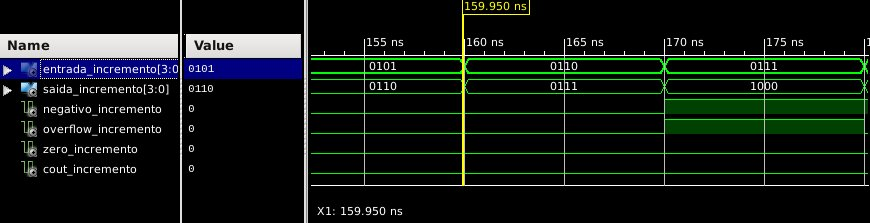
\includegraphics[scale=0.7]{testes/incremento.jpeg}
\caption{teste da função INCREMENTO}
\label{fig:diagrama}
\end{figure}

%%%%%%%%%%%%%%%%%%%%%%%%%%%%%%%%%%%%%%%%%%%%%%%%%%%%%%%%%%%%%%%%%%%%%%%%%%%%%%%%%%%%%%%
\section{Módulo ULA}
    Este módulo ULA recebe 2 entradas de 4 bits e um vetor de seleção (3 bits) que seleciona uma  entre as 8 opções de operações conforme a Tabela \ref{tabela1}.
    O módulo tem como saída o resultado(4 bits) da operação realizada resultado e suas flags correspondentes (OV , Neg, Cout, Zero).
    

\begin{table}[H]
\begin{tabular}{|c||c|} \hline
Seleção & Função \\\hline
000 & AND \\\hline
001 & OR\\\hline
010 & XOR\\\hline
011 & NOT \\\hline
100 & Somador de 4 bits \\\hline
101 & Subtrator de 4 bits \\\hline
110 & Complemento de 2 \\\hline
111 & Incremento \\\hline

\end{tabular}
\label{tabela1}
\centering
\caption{Seleção do vetor de 3 bits e sua respectiva função}
\label {tabela1}
\end{table}



\begin{lstlisting}
library IEEE;
use IEEE.STD_LOGIC_1164.ALL;

entity modulo_ULA is
    Port ( entrada_1_ula : in  STD_LOGIC_VECTOR (3 downto 0);
           entrada_2_ula : in  STD_LOGIC_VECTOR (3 downto 0);
           selecao : in  STD_LOGIC_VECTOR (2 downto 0);
           saida_ula : out  STD_LOGIC_VECTOR (3 downto 0);
           cout_ula : out  STD_LOGIC;
           zero_ula : out  STD_LOGIC;
           negativo_ula : out  STD_LOGIC;
           overflow_ula : out  STD_LOGIC);
end modulo_ULA;

architecture Behavioral of modulo_ULA is

------------------------------- Importando as funcoes
-- selecao = 000
component porta_and is
    Port ( entrada_1_and : in  STD_LOGIC_VECTOR (3 downto 0);
           entrada_2_and : in  STD_LOGIC_VECTOR (3 downto 0);
           resultado_and : out  STD_LOGIC_VECTOR (3 downto 0));
end component porta_and;


-- selecao = 001
component porta_or is
    Port ( entrada_1_or : in  STD_LOGIC_VECTOR (3 downto 0);
           entrada_2_or : in  STD_LOGIC_VECTOR (3 downto 0);
           resultado_or : out  STD_LOGIC_VECTOR (3 downto 0));
end component porta_or;

-- selecao = 010
component porta_xor is
    Port ( entrada_1_xor : in  STD_LOGIC_VECTOR (3 downto 0);
           entrada_2_xor : in  STD_LOGIC_VECTOR (3 downto 0);
           saida_xor : out  STD_LOGIC_VECTOR (3 downto 0));
end component porta_xor;

-- selecao = 011
component porta_not is
    Port ( entrada_not : in  STD_LOGIC_VECTOR (3 downto 0);
           saida_not : out  STD_LOGIC_VECTOR (3 downto 0));
end component porta_not;

-- selecao = 100
component somador_4bits is
    Port ( entrada_1_s4bits : in  STD_LOGIC_VECTOR (3 downto 0);
           entrada_2_s4bits : in  STD_LOGIC_VECTOR (3 downto 0);
           cin_s4bits : in  STD_LOGIC;
           cout_s4bits : out  STD_LOGIC;
           soma_s4bits : out  STD_LOGIC_VECTOR (3 downto 0);
           overflow_s4bits : out  STD_LOGIC;
           negativo_s4bits : out  STD_LOGIC;
           zero_s4bits : out  STD_LOGIC);
end component somador_4bits;

-- selecao = 101
component subtrator_4bits is
    Port ( entrada_1_subt4bits : in  STD_LOGIC_VECTOR (3 downto 0);
           entrada_2_subt4bits : in  STD_LOGIC_VECTOR (3 downto 0);
           borrow_in_subt4bits : in  STD_LOGIC;
           borrow_out_subt4bits : out  STD_LOGIC;
           resultado_subt4bits : out  STD_LOGIC_VECTOR (3 downto 0);
           zero_subt4bits : out  STD_LOGIC;
           negativo_subt4bits : out  STD_LOGIC;
           overflow_subt4bits : out  STD_LOGIC);
end component subtrator_4bits;


-- selecao = 110
component complemento_2 is
    Port ( entrada_compl2 : in  STD_LOGIC_VECTOR (3 downto 0);
           saida_compl2 : out  STD_LOGIC_VECTOR (3 downto 0));
end component complemento_2;


-- selecao = 111
component operacao_incremento is
    Port ( entrada_incremento : in  STD_LOGIC_VECTOR (3 downto 0);
           saida_incremento : out  STD_LOGIC_VECTOR (3 downto 0);
           negativo_incremento : out  STD_LOGIC;
           overflow_incremento : out  STD_LOGIC;
           zero_incremento : out  STD_LOGIC;
           cout_incremento : out  STD_LOGIC);
end component operacao_incremento;

-------------------------------- Auxiliares
signal aux_and, aux_or, aux_xor, aux_not :STD_LOGIC_VECTOR(3 downto 0);
signal aux_soma, aux_sub, aux_compl_2, aux_incrm :STD_LOGIC_VECTOR(3 downto 0);
signal cout_soma, bout_sub, cout_incrm : STD_LOGIC;
signal ov_soma, ov_sub, ov_incrm : STD_LOGIC;
signal neg_soma, neg_sub, neg_incrm : STD_LOGIC;
signal zero_soma, zero_sub, zero_incrm: STD_LOGIC;

begin
-------------------------------- Calculo das saidas auxiliares
-- 000
label0: porta_and port map (entrada_1_ula , entrada_2_ula, aux_and);
-- 001
label1: porta_or port map (entrada_1_ula , entrada_2_ula, aux_or);
-- 010
label2: porta_xor port map (entrada_1_ula , entrada_2_ula, aux_xor);
-- 011
label3: porta_not port map (entrada_1_ula , aux_not);
-- 100
label4: somador_4bits port map (entrada_1_ula, entrada_2_ula, '0', 
                    cout_soma, aux_soma, ov_soma,neg_soma, zero_soma);
-- 101
label5: subtrator_4bits port map (entrada_1_ula, entrada_2_ula, '0', 
                        bout_sub, aux_sub, zero_sub, neg_sub, ov_sub);
-- 110
label6: complemento_2 port map (entrada_1_ula, aux_compl_2);
-- 111
label7: operacao_incremento port map (entrada_1_ula, aux_incrm,
                 neg_incrm, ov_incrm, zero_incrm, cout_incrm);
							

-------------------------------- selecao das saidas principais
with selecao select
           saida_ula <=         aux_and     when "000" ,
                                aux_or      when "001" ,
                                aux_xor     when "010" ,
                                aux_not	    when "011" ,
                                aux_soma    when "100" ,
                                aux_sub	    when "101" ,
                                aux_compl_2 when "110" ,
                                aux_incrm   when others;
		
with selecao select
                cout_ula <=      '0'        when "000" ,
                                 '0'        when "001" ,
                                 '0'        when "010" ,
                                 '0'        when "011" ,
                                 cout_soma  when "100" ,
                                 bout_sub   when "101" ,
                                 '0'        when "110" ,
                                 cout_incrm when others;
		

with selecao select
          zero_ula <=            '0'        when "000" ,
                                 '0'        when "001" ,
                                 '0'        when "010" ,
                                 '0'        when "011" ,
                                 zero_soma  when "100" ,
                                 zero_sub   when "101" ,
                                 '0'        when "110" ,
                                zero_incrm when others ;


with selecao select
                   negativo_ula<= '0'       when "000" ,
                                  '0'       when "001" ,
                                  '0'       when "010" ,
                                  '0'       when "011" ,
                                  neg_soma  when "100" ,
                                  neg_sub   when "101" ,
                                  '0'       when "110" ,
                                  neg_incrm when others;
											
with selecao select
                   overflow_ula <= '0'      when "000" ,
                                   '0'      when "001" ,
                                   '0'      when "010" ,
                                   '0'      when "011" ,
                                   ov_soma  when "100" ,
                                   ov_sub   when "101" ,
                                   '0'      when "110" ,
                                   ov_incrm when others ;

end Behavioral;
} \end{lstlisting}

  \begin{figure}[H]
\centering
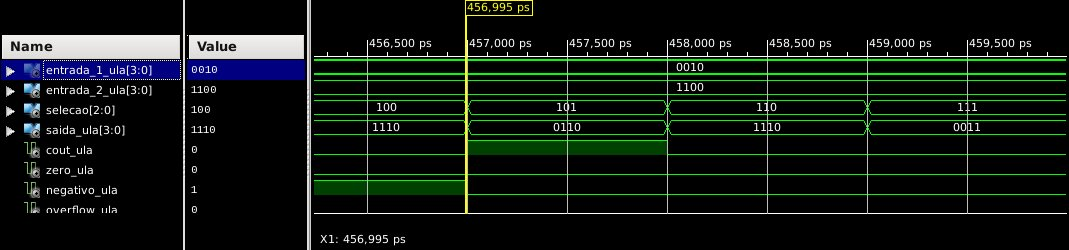
\includegraphics[scale=0.6]{testes/ula2.jpeg}
\caption{teste do MÓDULO ULA}
\label{fig:diagrama}
\end{figure}

%%%%%%%%%%%%%%%%%%%%%%%%%%%%%%%%%%%%%%%%%%%%%%%%%%%%%%%%%%%%%%%%%%%%%%%%%%%%%%%%%%%%%%%
\section{Módulo Principal}
O módulo principal será utilizado para tornar a ULA funcional na placa FPGA. Para isso vamos precisar ajustar o clock interno da placa e um gerador de entradas para suprir a falta de botões na placa.

\subsection{Redutor de Clock}
    Este módulo será usado para reduzir a frequência do clock interno à placa.
    Já que a frequência é de 50 MHz, vamos reduzir a frequência para 0,5 MHz para ser possível observar as operações acontecendo na placa. 
    
\begin{lstlisting}
library IEEE;
use IEEE.STD_LOGIC_1164.ALL;

entity redutor_clock is
    Port ( entrada_clock : in  STD_LOGIC;
           reset_clock : in  STD_LOGIC;
           saida_clock : out  STD_LOGIC);
end redutor_clock;

architecture Behavioral of redutor_clock is

signal contador : integer range 0 to 100_000_000 := 0;

  

begin
	transformadorfrequencia : process (entrada_clock, reset_clock)
	begin 
		if (reset_clock = '1') then
			contador <= 0;	
		elsif (entrada_clock'event and entrada_clock = '1') then
		
			if (contador < 50_000_000) then
				saida_clock <= '0';
			else
				saida_clock <= '1';
			end if;
					
			if (contador = 100_000_000) then
				contador <= 0;
			else
				contador <= (contador + 1);
			end if;
		end if;
			
	end process; 
		
end Behavioral;

} \end{lstlisting}
\subsection{Contador de 10 bits}
    Para gerar as entradas da ULA vamos criar um contador de 10 bits. Do segundo ao décimo bit iremos gerar as 2 entradas de 4 bits cada. Usaremos os 2 bits restantes para selecionar o que será mostrado nos leds (Entrada 1, Entrada 2, Resultado, Flags).

\begin{lstlisting}
library IEEE;
use IEEE.STD_LOGIC_1164.ALL;
use ieee.numeric_std.all;

entity contador_10bits is
    Port ( entrada_clock_contador_10bits, reset_contador_10bits : in  STD_LOGIC;
           saida_contador_10bits : out  STD_LOGIC_VECTOR (9 downto 0));
end contador_10bits;

architecture Behavioral of contador_10bits is
signal contador: INTEGER := 0;

begin

	contagem_10bits: process(entrada_clock_contador_10bits)

	begin 
	
		if (reset_contador_10bits = '1') then
			contador <= 0;
		elsif (entrada_clock_contador_10bits'event and  entrada_clock_contador_10bits = '1') then
			if (contador = 1023) then
				contador <= 0;
			else
				contador <= contador + 1;
			end if;
		end if; 	
		saida_contador_10bits <= STD_LOGIC_VECTOR(to_unsigned(contador,10));
	
	end process;
	
end Behavioral;

} \end{lstlisting}
\subsection{Módulo Principal}
    Com esse módulo, juntamos o redutor de clock e o contador de 10 bits para finalizar a ULA. Para o controle dos leds, os 2 bits restantes do contador irão seguir a (Tabela \ref{tabela2}). Além disso, o Módulo também receberá, como entrada, o vetor de 3 bits de seleção que será manipulado diretamente da placa.
    
\begin{table}[H]
\begin{tabular}{|c||c|} \hline
Seleção & Função \\\hline
00 &  Entrada 1 \\\hline
01 & Entrada 2 \\\hline
10 & Resultado \\\hline
11 & Flags \\\hline
 
\end{tabular}
\label{tabela2}
\centering
\caption{Seleção do vetor de 2 bits e sua respectiva função}
\label {tabela2}
\end{table}



\begin{lstlisting}
library IEEE;
use IEEE.STD_LOGIC_1164.ALL;

entity modulo_principal is
    Port ( entrada_clock_modulo_p : in  STD_LOGIC;
			  operacao_modulo_p : in STD_LOGIC_VECTOR (2 DOWNTO 0);
           saida_modulo_p : out  STD_LOGIC_VECTOR (3 DOWNTO 0);
			  saida_selecao_modulo_p : out  STD_LOGIC_VECTOR (1 DOWNTO 0));
end modulo_principal;

architecture Behavioral of modulo_principal is

component redutor_clock
    Port ( entrada_clock : in  STD_LOGIC;
           reset_clock : in  STD_LOGIC;
           saida_clock : out  STD_LOGIC);
end component;

component contador_10bits
    Port ( entrada_clock_contador_10bits, reset_contador_10bits : in  STD_LOGIC;
           saida_contador_10bits : out  STD_LOGIC_VECTOR (9 downto 0));
end component;

component modulo_ULA 
    Port ( entrada_1_ula : in  STD_LOGIC_VECTOR (3 downto 0);
           entrada_2_ula : in  STD_LOGIC_VECTOR (3 downto 0);
           selecao : in  STD_LOGIC_VECTOR (2 downto 0);
           saida_ula : out  STD_LOGIC_VECTOR (3 downto 0);
           cout_ula : out  STD_LOGIC;
           zero_ula : out  STD_LOGIC;
           negativo_ula : out  STD_LOGIC;
           overflow_ula : out  STD_LOGIC);
end component;


signal clock_reduzido : STD_LOGIC;
signal selecao_saida : STD_LOGIC_VECTOR (1 DOWNTO 0);
signal entrada_1, entrada_2 : STD_LOGIC_VECTOR (3 DOWNTO 0);
signal contador_auxiliar : STD_LOGIC_VECTOR (9 DOWNTO 0);
signal vetor_flags : STD_LOGIC_VECTOR (3 DOWNTO 0);
signal resultado_operacao : STD_LOGIC_VECTOR (3 DOWNTO 0);


begin

label0: redutor_clock port map(entrada_clock_modulo_p,'0', clock_reduzido);
label1: contador_10bits port map(clock_reduzido, '0', contador_auxiliar);

entrada_1 <= contador_auxiliar (9 downto 6);
entrada_2 <= contador_auxiliar (5 downto 2);
selecao_saida <= contador_auxiliar (1 downto 0);


label2: modulo_ULA port map (entrada_1, entrada_2, operacao_modulo_p, resultado_operacao, vetor_flags(0),
vetor_flags(1), vetor_flags(2), vetor_flags(3));

with selecao_saida select
                 saida_modulo_p<= entrada_1            when "00" ,
                                  entrada_2            when "01" ,
                                  resultado_operacao   when "10" ,
                                  vetor_flags          when others;
										

saida_selecao_modulo_p <= selecao_saida;


end Behavioral;

} \end{lstlisting}

\section{Conclusão}
    Com os códigos terminados, pudemos testar, simular e implementar na placa e observar seu funcionamento. Alguns problemas durante a implementação na placa foram analisados e consertados, tal como o carry in não estar em zero. Após consertar o erro, conseguimos encontrar os resultados desejados para cada operação da ULA.

\section{Bibliografia}
\begin{enumerate}
   \item https://www.gta.ufrj.br/ensino/EEL480/Introducao-VHDL.pdf
   \item https://www.gta.ufrj.br/ensino/EEL480/spartan3/ug334.pdf
   \item http://vhdl.renerta.com/mobile/source/vhd00027.htm
 \end{enumerate}



\end{document}
